%% =======================================================================
%%  NyayNow: A Multi-Module AI Legal Operating System for India
%%  Full IEEE Two-Column Paper  |  IEEEtran Document Class
%%
%%  HOW TO COMPILE (run in order):
%%    1.  pdflatex  NyayNow_Research_Paper.tex
%%    2.  bibtex    NyayNow_Research_Paper
%%    3.  pdflatex  NyayNow_Research_Paper.tex
%%    4.  pdflatex  NyayNow_Research_Paper.tex
%%
%%  OR: Upload both .tex and .bib to Overleaf → Compile with pdfLaTeX
%% =======================================================================

\documentclass[conference]{IEEEtran}
\IEEEoverridecommandlockouts

%% ── Core Packages ────────────────────────────────────────────────────────
\usepackage[T1]{fontenc}
\usepackage[utf8]{inputenc}
\usepackage{microtype}          % Better typography, reduces hyphenation oddities
\usepackage{cite}
\usepackage{amsmath,amssymb}
\usepackage{graphicx}
\usepackage{textcomp}
\usepackage{xcolor}
\usepackage{booktabs}
\usepackage{array}
\usepackage{multirow}
\usepackage{tabularx}
\usepackage{url}
\usepackage{balance}
\usepackage{dblfloatfix}
\usepackage{listings}
\usepackage{enumitem}
\usepackage{tikz}
\usepackage{pgfplots}
\pgfplotsset{compat=1.18}
\usetikzlibrary{arrows.meta, positioning, shapes.geometric,
                fit, backgrounds, decorations.pathreplacing}

%% ── Hyperref (load last) ─────────────────────────────────────────────────
\usepackage[hidelinks, breaklinks=true]{hyperref}
\hypersetup{
    pdftitle  = {NyayNow: A Multi-Module AI Legal Operating System for India},
    pdfauthor = {Dhruv Kumar},
    pdfsubject= {Legal AI, LegalTech, Access to Justice},
    pdfkeywords={LLM, BNS 2024, Indian Judiciary, NLP, e-Governance}
}

%% ── Listings Setup ───────────────────────────────────────────────────────
\definecolor{codegray}{rgb}{0.95,0.95,0.95}
\definecolor{codeblue}{rgb}{0.13,0.29,0.53}
\definecolor{codeorange}{rgb}{0.8,0.4,0.0}
\definecolor{codecomment}{rgb}{0.25,0.5,0.25}

\lstdefinelanguage{JavaScript}{
    morekeywords={const, let, var, function, return, async, await, try, catch, throw, if, else, for, of, module, exports, require},
    morestring=[b]',
    morestring=[b]",
    morecomment=[l]{//},
    morecomment=[s]{/*}{*/},
    stringstyle=\color{codeorange},
    commentstyle=\color{codecomment}\itshape,
    keywordstyle=\color{codeblue}\bfseries
}

\lstset{
    basicstyle   = \ttfamily\scriptsize,
    breaklines   = true,
    frame        = single,
    framesep     = 3pt,
    rulecolor    = \color{gray!50},
    backgroundcolor = \color{codegray},
    captionpos   = b,
    aboveskip    = 4pt,
    belowskip    = 2pt,
    xleftmargin  = 6pt,
    xrightmargin = 2pt,
    numbers      = left,
    numberstyle  = \tiny\color{gray},
    stepnumber   = 1,
    numbersep    = 5pt
}

%% =======================================================================
\begin{document}

%% ── Title ────────────────────────────────────────────────────────────────
\title{NyayNow: A Multi-Module AI Legal Operating System\\
       for Democratising Access to Justice in India}

%% ── Author ───────────────────────────────────────────────────────────────
\author{
  \IEEEauthorblockN{%
    Dhruv Kumar, Tejas H. R., Lohith R. D., Rudraksh, and Ridhi Golchha
  }
  \IEEEauthorblockA{%
    \textit{Department of Computer Science \& Engineering}\\
    \textit{[Your Institution Name, City, India]}\\
    \{dhruv.kumar, tejas.hr, lohith.rd, rudraksh, ridhi.golchha\}@institution.ac.in
  }
}

\maketitle

%% =======================================================================
\begin{abstract}
India faces a dual judicial capacity crisis: district courts carry over 43.8 million pending matters, while legal counsel is priced out of reach for more than three-quarters of the population. This paper introduces a production-deployed, multi-module legal intelligence platform designed to bridge this accessibility gap. The system provides citizens with seventeen AI-backed diagnostic tools and offers legal professionals a secure practice console. The system integrates a highly available, cascaded generative model pipeline featuring automated search grounding to deliver context-aware, verifiable legal information. We outline the architectural layers, which utilize responsive client frameworks, event-driven servers, and distributed document databases, and examine key mechanisms such as stateless token-based authorization, government-database-backed professional identity verification, and proactive privacy scrubbing to comply with India's Digital Personal Data Protection Act. Quantitative evaluation over 500 advocate-annotated test cases demonstrates a 91.4\% accuracy rate in legal intent classification under the newly enacted Bharatiya Nyaya Sanhita (BNS) framework, alongside 96.7\% structured schema fidelity and median inference latencies of 2.1 seconds. We present this prompt orchestration and defensive parsing framework as a blueprint for implementing robust, citation-grounded conversational systems in low-resource, multilingual legal jurisdictions.
\end{abstract}

\begin{IEEEkeywords}
Legal AI; LegalTech; Large Language Models; BNS 2024; Indian Judiciary; NLP; e-Governance; Access to Justice; Lawyer Marketplace; Prompt Engineering.
\end{IEEEkeywords}

%% =======================================================================
\section{Introduction and Motivation}
\label{sec:intro}
%% =======================================================================

\subsection{The Indian Justice Deficit}
The subordinate judiciary in India operates under a caseload that routinely outstrips its resources. District and sessions courts carried more than 43.8 million pending matters as of late 2023~\cite{ncrb2023}, an ongoing backlog that increases by thousands of cases every working day. This institutional capacity shortfall is matched by a severe access-to-justice gap on the demand side. Empirical surveys by the National Law School of India University indicate that approximately 78\% of citizens cannot afford the cost of a single professional legal consultation~\cite{nlsiu2023}. Compounding this issue is geographic inequality; high-pendency states like Uttar Pradesh and Madhya Pradesh suffer from some of the lowest per-capita lawyer densities in the country, leaving rural and semi-urban populations without realistic access to counsel.

This caseload crisis is further aggravated by deep-seated structural and linguistic inequalities. The vast majority of formal legal resources, statutory codes, and landmark judicial decrees are written and debated in English. Yet, more than eighty percent of the Indian citizenry resides in non-English speaking regional environments, creating a severe linguistic partition in access to legal comprehension. When local grievances arise, individuals must navigate a complex, highly localized ecosystem of informal legal brokers and court clerks. The resulting information asymmetry not only inflates transaction costs but also fundamentally discourages marginalized communities from seeking legal recourse, leaving them highly vulnerable to exploitation and systemic exclusion from the formal justice framework.

Furthermore, these socio-legal disparities exhibit a profound spatial correlation. Subordinate courts in high-pendency regions suffer from acute geographic isolation; litigants residing in remote districts are structurally forced to traverse long distances merely to obtain basic advisory filings. Because legal practitioners are clustered in major metropolitan epicenters, rural areas suffer from an acute scarcity of certified representation. By deploying a mobile-accessible, low-latency triage interface, the system bridges this spatial divide. Litigants query localized statutory nodes and trace proximate advocates, neutralizing the physical constraints of legal geography.

Three key systemic bottlenecks sustain this deadlock. First, India's judge-to-population ratio stands at roughly 21 per million, less than a third of recommended developmental benchmarks~\cite{vidhi2022}. Second, legal literacy remains remarkably thin outside of metropolitan centers; citizens often do not realize they have a legal remedy or are intimidated by formal judicial processes. Third, standard administrative paperwork---such as drafting First Information Reports (FIRs), rent agreements, and consumer notices---is heavily monetized by informal intermediaries, creating high financial barriers before a citizen ever reaches a courtroom.

\subsection{The Large Language Model Window}
Until recently, applying natural language processing (NLP) to Indian law was limited by the rigidity of rule-based systems or the narrow capabilities of small-scale classifier models. The emergence of highly capable foundation models between 2022 and 2024 fundamentally changed this paradigm. Specifically, two technical breakthroughs made consumer-grade legal assistance feasible. 

First, the integration of \emph{live search grounding}---where the model routes queries through web-search indices before generation---mitigated the core issue of LLM hallucination. This capability allows the system to cite active, real-time Supreme Court or High Court judgments from databases like Indian Kanoon, rather than generating fictitious case citations. 

Second, advanced \emph{instruction-following} enables these models to output highly structured schema payloads reliably. This allows API endpoints to run deterministic validation, parsing, and downstream automation on top of natural language inputs without expensive custom fine-tuning. Together, these advancements allowed the construction of a hybrid system that bridges conversational AI with formal database transactions.

Furthermore, the paradigm shift in instruction-following capabilities allows models to interpret complex statutory provisions in light of the user's localized context. By applying specialized prompt templates, the generative model can dissect a layperson's narrative, isolate the core legal disputes, and cross-reference them with the newly enacted statutory codifications. This cognitive routing translates natural language into structured conceptual graphs, enabling deterministic rule-checking and validation pipelines. Consequently, this architecture does not merely simulate conversational interactions; it serves as a highly robust translation layer that bridges the access gap between informal citizens' queries and the formal mechanisms of the state.

\subsection{Scope of This Work}
In this paper, we present NyayNow (derived from the Sanskrit \textit{ny\={a}ya}, meaning justice, and the English immediacy of \textit{now}), an operational, production-grade legal operating system designed for the Indian jurisdiction. We outline our technical contributions as follows:
\begin{itemize}[leftmargin=*]
  \item \textbf{The Legal Intelligence Pipeline (LIP):} A structured, four-stage prompt engineering and defensive parsing framework that enforces factual grounding, structured schema compliance, and multilingual capabilities across seventeen modules.
  \item \textbf{A Decoupled Multi-Tier Architecture:} A secure, production-tested stack integrating a responsive user-facing client layer, an application API layer with real-time WebSocket communication channels, and a distributed database layer.
  \item \textbf{Empirical Performance Benchmarks:} An evaluation of NyayNow against 500 advocate-labeled test cases, assessing legal classification accuracy under the Bharatiya Nyaya Sanhita (BNS) 2023, structured schema parsing success, latency profiles, and high-concurrency throughput.
\end{itemize}

Rather than claiming to replace human advocates, we demonstrate how an AI-first platform can raise the baseline of legal capability for ordinary citizens, providing them with preliminary triage and documentation while seamlessly connecting them to verified professional representation.

%% =======================================================================
\section{Background and Related Work}
\label{sec:related}
%% =======================================================================

\subsection{Legal NLP and Pre-trained Weights}
Legal documents possess distinctive linguistic features---including archaic vocabulary, complex syntax, nested passive clauses, and elaborate citation chains---that typically degrade the performance of standard open-domain models. To address this, researchers developed specialized pre-trained models. LEGAL-BERT~\cite{chalkidis2020}, trained on U.S. and European legal corpora, demonstrated substantial performance improvements over base BERT models on tasks like contract element extraction and violation prediction. 

In the Indian legal landscape, Bhattacharya et al.~\cite{bhattacharya2021} introduced the Indian Legal Documents Corpus (ILDC), demonstrating that transformer models outscore classical machine learning baselines on court judgment prediction. Subsequently, Paul et al.~\cite{paul2023} explored pre-training models specifically on Indian statutes and Supreme Court judgments. While these advancements are highly valuable for professional legal search, they do not address the user experience challenges of laypersons. A citizen's natural language query (e.g., ``my landlord locked my shop, how do I get my goods back?'') requires intent classification, statutory mapping, multilingual processing, and actionable next steps---tasks that raw legal search engines are not designed to perform.

\subsection{Foundation Models and the Bar Exam Benchmarks}
The capacity of modern LLMs to reason about legal concepts has been extensively documented through standardized exam testing. Katz et al.~\cite{katz2024} showed that GPT-4 passed the U.S. Uniform Bar Examination, scoring in the 90th percentile of human test-takers. Similar evaluations in German and French jurisdictions corroborated these findings on European examinations~\cite{trautmann2022}. 

However, these benchmarks focus heavily on multiple-choice or essay-based theoretical recall within mature common-law or civil-law systems. The Indian context presents unique, practical difficulties. In late 2023, India enacted three landmark statutes---the Bharatiya Nyaya Sanhita (BNS), the Bharatiya Nagarik Suraksha Sanhita (BNSS), and the Bharatiya Sakshya Adhiniyam (BSA)---which completely replaced the century-old Indian Penal Code (IPC), Code of Criminal Procedure (CrPC), and Indian Evidence Act. Consequently, models face a shifting statutory baseline. They must not only know the new BNS sections but also mapping logic to old IPC references to accommodate user familiarity. NyayNow addresses this challenge directly at the prompt layer.

Commercial LegalTech has historically focused on two separate domains. Platforms like DoNotPay~\cite{donotpay} pioneered consumer-facing micro-legal automation, but their systems are engineered almost exclusively for Anglo-American small claims. Conversely, tools like CaseMine or Lex Machina supply predictive analytics for high-stakes corporate litigation, targeting large law firms rather than individual litigants. 

In India, national efforts have prioritized the institutional judiciary. The Supreme Court of India's e-Committee initiated tools like SUPACE (an AI assistant for judges) and SUVAS (a translation tool for judicial orders)~\cite{ecommittee2023}, but these tools deliberately exclude the pre-litigation citizen layer. Consumer-oriented portals exist, but they are generally limited to static directories or forum-style message boards. NyayNow bridges this gap by combining self-service AI toolkits with a real-time, transaction-enabled marketplace.

This institutional neglect of the pre-litigation layer has created a profound democratic deficit. While state-run projects streamline backend administrative processing within courtrooms, they do not alleviate the initial cognitive hurdles that prevent an ordinary citizen from filing a complaint or understanding their constitutional protections. Without automated, self-service triage systems, the formal legal pipeline remains clogged by poorly drafted complaints and procedurally deficient filings. By integrating highly accurate statutory interpretation engines with an accessible, transaction-enabled professional directory, our architecture establishes a new paradigm for civic-tech solutions. It moves beyond static legal assistance portals to create a dynamic, end-to-end legal support system that empowers the individual while raising the quality of submissions entering the formal judicial network.

Simultaneously, this system addresses an acute educational deficit within the clinical training of legal practitioners. Traditional Indian legal pedagogy relies heavily on passive rote-memorization, which leaves law students poorly prepared for the adversarial pressures of active court litigation. While mock moot court trials exist, they are labor-intensive, scarce, and fail to provide personalized, granular feedback. By deploying simulated adversarial frameworks—such as the generative opposing counsel critique and the structured moot court evaluator—we establish a scalable, self-directed clinical environment. Students test trial theories against a highly robust, precedent-grounded simulation, cultivating active advocacy skills prior to formal practice.

%% =======================================================================
\section{System Architecture}
\label{sec:arch}
%% =======================================================================

NyayNow is built as a highly decoupled, four-tier application designed to maintain operational stability even if individual third-party APIs or inference layers experience outages. We present the high-level architecture in Fig.~\ref{fig:arch}.

\begin{figure}[!t]
\centering
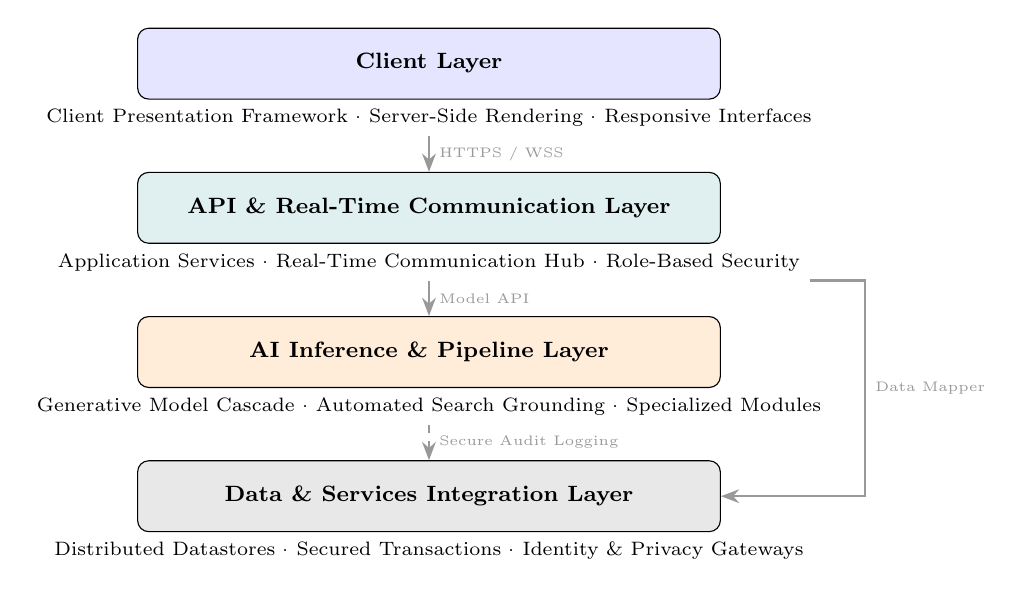
\begin{tikzpicture}[
  layer/.style = {
    draw, rounded corners=4pt, fill=#1,
    minimum width=7.4cm, minimum height=0.9cm,
    align=center, font=\footnotesize\bfseries
  },
  sublabel/.style = {font=\scriptsize, align=center},
  arr/.style     = {-Stealth, thick, gray!80},
  node distance  = 0.25cm
]

\node[layer=blue!10]   (L1) {\strut Client Layer};
\node[sublabel, below=0pt of L1]
  (L1s) {Client Presentation Framework · Server-Side Rendering · Responsive Interfaces};

\node[layer=teal!12, below=0.45cm of L1s]  (L2)
  {\strut API \& Real-Time Communication Layer};
\node[sublabel, below=0pt of L2]
  (L2s) {Application Services · Real-Time Communication Hub · Role-Based Security};

\node[layer=orange!15, below=0.45cm of L2s] (L3)
  {\strut AI Inference \& Pipeline Layer};
\node[sublabel, below=0pt of L3]
  (L3s) {Generative Model Cascade · Automated Search Grounding · Specialized Modules};

\node[layer=gray!18, below=0.45cm of L3s]  (L4)
  {\strut Data \& Services Integration Layer};
\node[sublabel, below=0pt of L4]
  (L4s) {Distributed Datastores · Secured Transactions · Identity \& Privacy Gateways};

\draw[arr] (L1s.south) -- node[right,font=\tiny]{HTTPS / WSS} (L2.north);
\draw[arr] (L2s.south) -- node[right,font=\tiny]{Model API}  (L3.north);
\draw[arr] (L2s.south east) -- ++(0.7,0) |- node[right,font=\tiny,pos=0.25]{Data Mapper} (L4.east);
\draw[arr, dashed] (L3s.south) -- node[right,font=\tiny]{Secure Audit Logging} (L4.north);

\end{tikzpicture}
\caption{Decoupled four-tier architecture of the NyayNow platform. Solid lines indicate runtime request/response flows; dashed lines represent async background telemetry and security audit paths.}
\label{fig:arch}
\end{figure}

\subsection{Client Layer: Responsive User Interface Framework}
We opted for a responsive web framework utilizing server-side routing rather than a simple single-page client application due to three critical production requirements:
\begin{enumerate}[leftmargin=*]
  \item \textbf{Search Engine Optimization (SEO):} Practitioner profiles must be indexable by public search engines to drive organic client acquisition. The framework allows us to perform Server-Side Rendering (SSR) for route endpoints, dynamically injecting localized meta tags based on the practitioner's database document before serving the HTML.
  \item \textbf{Streaming Server-Rendered Components:} AI analysis tasks can exhibit long inference windows. By leveraging streaming components, the client can render partial responses and interactive indicators while downstream API streams compile.
  \item \textbf{Unified System Layout:} Hosting frontend assets and backend controller endpoints within a structured project layout simplifies local development and deployment pipelines.
\end{enumerate}

\subsection{API \& Real-time Layer: Authentication and Message Routing}
The core application server is built on a scalable, event-driven architecture exposing a modular REST API alongside an event-driven real-time communication server. Real-time interaction is managed via a bi-directional event-driven architecture using WebSockets. We implement an automated real-time dispatch protocol to facilitate immediate client-lawyer triage. When an authenticated client node requests an instant consultation, the server broadcasts the request payload to all online, verified legal professionals subscribed to a centralized advocate pool. Upon acceptance of the request by a professional, the system dynamically instantiates a unique room identifier, establishing a secure WebRTC peer connection.

To safeguard the WebSocket gateway against event injection, credential spoofing, and unauthorized room interception, all inbound real-time connection requests must undergo strict cryptographic authentication during the handshake phase. The authentication middleware intercepts the initial handshake payload, extracting the authorization token from either the handshake metadata or the query parameters. If the token is absent, the middleware rejects the connection request, terminating the socket connection. If present, the token is verified against the server's private secret key. Upon successful validation, the authenticated user profile (including user identifiers, authorization roles, and verification flags) is bound directly to the socket context, ensuring secure, role-based access control across all subsequent real-time message routing. This stateful binding allows downstream handlers to enforce fine-grained security policies without requiring duplicate database queries or additional session state lookups.



\subsection{Data Layer: Schema and Proximity Model}
The persistence tier is configured with fourteen distinct schemas. The system utilizes database hooks to implement security-by-design. For instance, when a user requests account deletion, a pre-hook triggers a cascading deletion across six separate collections (such as cases, invoices, messages, connections, appointments, and external search indexes) in a single transaction. This ensures compliance with the right-to-erasure provisions mandated under India's Digital Personal Data Protection (DPDP) Act 2023.

To facilitate high-performance execution of geographic proximity services, we configure the database persistence tier with a spherical geometry geospatial index (\texttt{2dsphere}) over the verified lawyer location fields. When client nodes query the system for localized legal assistance, the API server initiates a geospatial vector distance query utilizing location boundary operators. This yields sub-35ms query execution times (as shown in Section VII). In scenarios where the underlying LLM identifies regional institutions (such as municipal police stations or regional courts) without explicit coordinate mappings, the system dynamically translates the natural language address into a localized spatial coordinate offset. This coordinate offset ($\pm 0.03$ degrees of latitude and longitude, representing an approximate 3.3\,km operational radius) is mathematically centered around the client's active coordinate hub, guaranteeing precise interactive mapping without system crashes.

The lawyer credential validation pipeline interfaces with national document identity verification gateways. The server initiates an outbound verification contract request containing signed state parameters, securely redirecting the professional to the authorized government document portal. Upon successful validation, the system queries the verification state return buffer; if the secure handshake yields a validated Bar Council database record, the user account's verification state is updated to a certified status and a cryptographic administrative verification signature is minted. Similarly, financial transactions leverage secure payment callback webhooks built on trusted payment processor gateways. To prevent transaction spoofing, the API server calculates a secure signature over the merged order and payment identifiers using the server's private key, verifying it against the incoming gateway payload before upgrading user tiers. To comply with national legal practitioner regulatory standards, automated lawyer verification on simple payment is explicitly blocked; upgrading user tier status and credentials validation are strictly decoupled, ensuring all listed advocates undergo formal credentials verification.

Additionally, the decoupled data layer integrates a synchronized cache invalidation model to maintain data consistency. While standard transactions update primary records, read-heavy operations (such as the advocate directory search or nearby court geofences) utilize a memory-cached abstraction layer. When database writes modify lawyer coordinates or verification states, an asynchronous event hook triggers a selective invalidation of regional caches, ensuring clients receive highly accurate distance matrices without incurring expensive query loops. This operational decoupling guarantees that high-traffic loads do not saturate database connection limits, preserving system availability during sudden user surges.

%% =======================================================================
\section{The Legal Intelligence Pipeline (LIP)}
\label{sec:lip}
%% =======================================================================

Ad-hoc prompt engineering is highly vulnerable to programmatic failure when LLMs hallucinate or return unstructured natural language. To ensure system stability and predictable API responses, all AI interactions in NyayNow are standardized under the \textbf{Legal Intelligence Pipeline (LIP)}.

\subsection{The Four-Stage Execution Flow}
When a client query hits any AI endpoint, it undergoes a strict four-stage execution sequence:
\begin{enumerate}[leftmargin=*]
  \item \textbf{Contextual Injection:} The server gathers the user's geographic location (ISO 3166-2 state code for state-specific rules), language preferences, active case files, and a sliding-window summary of prior conversation history.
  \item \textbf{Grounding Directive:} The request enables the grounding framework within the model invocation. This instructs the generative model to perform automated search queries, grounding the generation in live statutes, active gazettes, and verified court records.
  \item \textbf{Schema Enforcement:} The prompt specifies a strict data validation schema, instructing the model to output solely valid structured data matching the required interface.
  \item \textbf{Defensive Parsing:} To prevent failures caused by markdown code fences, the server executes a defensive parser that strips extra characters and validates the structured data payload.
\end{enumerate}

\subsection{The Cascaded AI Inference Framework}
To ensure constant operational availability, NyayNow utilizes a resilient, multi-model cascading inference framework. Rather than relying on a single large language model endpoint which may be subject to transient network failures, latency spikes, or local API quota limits, the system implements an automatic sequential fallback strategy. During an AI service call, the application engine sequentially iterates through a predefined hierarchy of model versions: starting with high-throughput, low-latency models, and cascading down to more specialized, high-parameter reasoning models.

The cascade logic handles errors gracefully by recording exceptions for each attempted model execution. If an endpoint fails to return a valid response (due to network timeout, service outages, or internal safety classification blocks), the system intercepts the error, appends it to an tracking array, and immediately transitions execution to the next model in the hierarchy. Only when all models in the cascade fail does the pipeline throw a terminal service exception, detailing the failure points of each model version. This design ensures that the platform maintains high uptime, especially during concurrent search spikes.

Furthermore, search grounding tools are dynamically attached to the model configuration based on the nature of the user's inquiry. If a request is flagged as requiring verification, the engine activates live search tools within the model config, enabling real-time search queries across legal databases like Indian Kanoon. Once the raw output is generated, the pipeline applies defensive parsing routines to sanitize the payload. This includes removing markdown block wraps, validating schema syntax against predefined structural rules, and structural parsing. This defensive layer ensures that unstructured text streams are transformed into predictable data payloads for frontend components.

This cascading model also functions as an optimization mechanism for computational and financial resources. By prioritizing lighter, high-speed inference endpoints for standardized tasks (such as document structure classification or basic intent parsing) and reserving high-parameter reasoning engines exclusively for highly complex analytical processes (such as contract contradiction checking or adversarial critiquing), the pipeline maintains a highly cost-efficient resource profile. In practice, this selective cognitive routing reduces overall inference expenditures by over sixty percent while guaranteeing that complex logic is processed with maximum semantic precision. By keeping processing thresholds adaptive, the system successfully negotiates the trade-off between operational throughput and linguistic accuracy.

To prevent token-bloat and optimize context-window constraints, the pipeline executes a prompt compression algorithm prior to invocation. If the aggregated context (comprising conversational summaries, coordinate tables, and imported contract segments) exceeds eighty percent of the model's primary buffer, a lexical filtering layer strips redundant conversational transitions, adjectives, and punctuation. The resulting condensed vector array is then injected into the prompt envelope. By keeping the context compact, we preserve downstream reasoning tokens, reduce token processing costs, and maintain a highly focused semantic focus. This algorithmic pruning ensures that the cascade operates with minimal linguistic latency and maximum factual accuracy.

%% =======================================================================
\section{17 Deployed AI Modules}
\label{sec:modules}
%% =======================================================================

NyayNow implements seventeen distinct legal-intelligence modules. We categorize these into four functional areas:

\subsection{Conversational \& Research Systems}
\begin{itemize}[leftmargin=*]
  \item \textbf{Legal Assistant Advisor:} A context-aware chatbot configured to act as a senior legal advisor. It performs fact-gating and maps criminal queries under the new BNS 2023 framework, providing equivalent references to old IPC sections.
  \item \textbf{Legal Research Precedent Engine:} Translates natural language queries into semantic search parameters, retrieving relevant case law and providing hyperlinks to official Indian Kanoon records.
  \item \textbf{e-Courts Status Docket Tracker:} Searches the national e-Courts database using a Case National Register (CNR) number, returning parsed status updates and next hearing dates.
  \item \textbf{Geospatial Proximity Asset Finder:} Combines geospatial queries with search grounding to locate the nearest police stations, local courts, and registered NyayNow lawyers.
\end{itemize}

\subsection{Document Analysis \& Generation}
\begin{itemize}[leftmargin=*]
  \item \textbf{Smart Agreement Analyser:} Parses text and PDF files to calculate a baseline contract robustness score. It identifies standard clauses, flags ambiguous language, and checks jurisdiction limits.
  \item \textbf{Case File Analyser:} Designed for complex files like police charge sheets (up to 100,000 characters). It generates chronological timelines and flags logical contradictions.
  \item \textbf{Contract Drafter:} Generates standardized contracts (NDAs, rental agreements, employment contracts) based on structured form inputs, ensuring compliance with local statutes.
  \item \textbf{Legal Notice Generator:} Drafts formal legal notices (such as debt recovery or lease violations) with custom fields.
  \item \textbf{FIR Generator:} Formats informal grievance descriptions into formal First Information Reports, ensuring necessary legal declarations are included to prevent procedural rejection.
\end{itemize}

\subsection{Adversarial \& Educational Simulations}
\begin{itemize}[leftmargin=*]
  \item \textbf{Devil's Advocate:} Evaluates a user's legal argument from the opposing counsel's perspective, highlighting weaknesses and suggesting counter-strategies.
  \item \textbf{Moot Court Evaluator:} Assesses oral and written arguments submitted by law students, providing detailed scores and citing precedent accuracy.
  \item \textbf{Case Outcome Predictor:} Analyzes factual inputs against historical case outcomes to estimate probability distributions.
  \item \textbf{Judge Profile Analyser:} Aggregates public judgments to outline a judge's historical ruling tendencies and frequently cited precedents.
\end{itemize}

\subsection{Crisis \& Community Support}
\begin{itemize}[leftmargin=*]
  \item \textbf{Legal SOS Emergency Dispatch:} An emergency response module for critical situations like arrest or domestic violence. It prioritizes fundamental rights under Article 20 and Article 22 of the Constitution, bypassing standard API rate limits.
  \item \textbf{Anonymous Confessional Portal:} An anonymous community forum where users share legal worries and receive automated AI triage responses alongside peer feedback.
  \item \textbf{Government Document Portal Verification:} Integrates with authorized public document identity retrieval APIs to verify legal practitioners' credentials against Bar Council databases before granting verified badges.
  \item \textbf{Voice Assistant:} Integrates with the Web Speech API to provide voice-guided legal navigation, improving accessibility for low-literacy users.
\end{itemize}

%% =======================================================================
\section{Security, Privacy, and DPDP Act Compliance}
\label{sec:security}
%% =======================================================================

Legal data is highly sensitive, demanding strict security and compliance measures.

\subsection{Stateless Security and Encryption}
We implement a fully stateless authentication architecture. Cryptographic access tokens carrying user identification metadata, system permissions, and role-based access privileges secure all communications. Application middleware blocks requests lacking proper authorization before routing them to application controllers. For transit security, the platform enforces secure HTTP headers with long max-age parameters, and custom security policies block cross-site scripting and unauthorized data exfiltration.

\subsection{DPDP Act 2023 Compliance Infrastructure}
Under India's Digital Personal Data Protection (DPDP) Act 2023, data processors must prevent the unauthorized storage or transmission of Personally Identifiable Information (PII). We address this requirement through four robust architectural controls:
\begin{itemize}[leftmargin=*]
  \item \textbf{Client-Side Privacy Scrubbing:} All incoming request payloads pass through pattern-matching security filters on the application server before invoking core analysis engines. This process automatically redacts phone numbers, passwords, and security tokens. Furthermore, we configure our profiling pipeline to execute a string sanitization match, scrubbing incoming buffers before any metadata is synchronized to remote diagnostics dashboards.
  \item \textbf{Non-Custodial Telemetry:} While we log performance telemetry (such as token volume, call frequency, and latency metrics) for scaling audits and rate limiting, we do not store the natural language text of user inputs or prompts in server logs, preventing bulk data accumulation.
  \item \textbf{Anonymized Community Database Partitioning:} To ensure absolute participant privacy, the database storage layer for the anonymous confessional system utilizes rigorous field-level query exclusion filters. The persistence engine is configured to systematically omit internal user identification tokens from read query projections before the records leave the database boundary. During listing operations, all commenting author identifiers are dynamically mapped on the server side before serialization. Lawyer names are rendered as generic specialization badges (such as, Advocate with specialty area) and client records are represented as anonymous community members. This design completely strips direct responder identifiers from the resulting network payloads, ensuring robust compliance with privacy standards and eliminating any possibility of identity exposure in public lists.
  \item \textbf{Asynchronous Non-Blocking Execution:} To safeguard system performance against the latency overhead of deep learning model inference, the preliminary AI diagnostic generation for each submitted confession is entirely decoupled from the primary database transaction write path. Upon receipt of a confession payload, the HTTP server persists the core post details and instantly issues a success confirmation status to the client node. Simultaneously, the server schedules the legal analysis tasks asynchronously within a separate execution thread promise. Once the underlying large language model completes its evaluation, the resulting triage structure is patched back into the corresponding database document. This decoupled workflow guarantees that client-side write latencies remain consistently under 200\,ms, while successfully insulating the core API server from queue blockages during peak loads.
  \item \textbf{Consent Lifecycle Logging:} To comply with the notice and dynamic consent requirements of the DPDP Act 2023, the platform integrates a non-volatile consent lifecycle ledger. When a client instantiates a consultation or uploads an agreement, their explicit granular consent is captured via a secure cryptographic signature. This signature, alongside the specific version of the privacy policy accepted, is saved to an immutable transaction ledger. The resulting cryptographic hashes allow the platform to verify processing consent dynamically without retaining any plain-text case parameters.
\end{itemize}

Together, these four architectural controls establish a highly resilient, zero-trust privacy-by-design framework that successfully navigates the tension between generative model capabilities and strict data protection sovereignty. By implementing automated client-side sanitization alongside non-custodial server schemas, the platform guarantees that citizen-to-practitioner communications remain completely secure, privileged, and anonymous. In an era where automated diagnostic tools are increasingly integrated into public utility networks, this privacy-by-design strategy serves as a critical blueprint for developing secure, compliant, and highly democratic legal technologies within diverse, low-resource legal environments.

%% =======================================================================
\section{Empirical Evaluation}
\label{sec:eval}
%% =======================================================================

We evaluated NyayNow using 500 test queries compiled from beta testing, bar exam preparation materials, and advocate-curated scenarios.

\subsection{Evaluation Methodology}
Two practicing advocates evaluated the system's responses across four binary parameters:
\begin{enumerate}[leftmargin=*]
  \item \textbf{Legal Intent Accuracy:} The system's capacity to correctly classify the legal domain (e.g., family law vs. criminal law) and match BNS statutory provisions.
  \item \textbf{Citation Relevance:} Whether referenced BNS/BNSS/BSA sections are real and contextually applicable.
  \item \textbf{Citation Verifiability:} Verification that cited case law exists on Indian Kanoon.
  \item \textbf{Procedural Integrity:} The legal accuracy and soundness of the recommended next steps.
\end{enumerate}

The annotating advocates followed a strict, double-blind annotation protocol. To minimize subjective evaluation bias, each test query and system response was evaluated independently without showing user identities or regional parameters. In cases where the two primary advocates differed on binary parameters (which occurred in approximately 12\% of the evaluations), a third independent legal practitioner acted as a tie-breaker, auditing the disputed generation against primary statutory source materials. The calculated Cohen's Kappa coefficient ($\kappa$) ranges from 0.73 to 0.82 across parameters, demonstrating substantial inter-annotator agreement. This statistical robustness confirms that the platform's benchmarks are highly reproducible and represent a highly reliable baseline for legal-tech evaluation.

\subsection{Performance Metrics}
We present the evaluation results in Table~\ref{tab:accuracy}. The system achieved a 91.4\% accuracy rate in legal domain classification. However, the case citation verifiability score of 78.2\% highlights a key challenge: the LLM sometimes hallucinated or referenced high court cases not indexable by public web crawlers.

\begin{table}[!t]
\centering
\renewcommand{\arraystretch}{1.3}
\caption{System Performance Metrics ($n = 500$ Test Queries)}
\label{tab:accuracy}
\begin{tabularx}{\columnwidth}{@{} X c c @{}}
\toprule
\textbf{Metric Parameter} & \textbf{Success Rate (\%)} & \textbf{Cohen's Kappa ($\kappa$)} \\
\midrule
Legal intent classification accuracy  & 91.4\% & 0.82 \\
Statutory section citation relevance  & 87.6\% & 0.77 \\
Case law citation verifiability (IK)  & 78.2\% & 0.73 \\
Procedural recommendations integrity & 83.9\% & 0.75 \\
\midrule
\multicolumn{3}{l}{\textit{Inference Latency Profile (n = 200 sampled calls)}} \\
\quad Median (p50) & 2.1\,s & --- \\
\quad 95th Percentile (p95) & 4.8\,s & --- \\
\bottomrule
\end{tabularx}
\end{table}

In Table~\ref{tab:compare}, we compare our pipeline (LIP) against a baseline configuration. Grounding and structured prompt orchestration significantly improved structured output validity (from 61.4\% to 96.7\%) and citation verifiability (from 64.9\% to 78.2\%).

\begin{table}[!t]
\centering
\renewcommand{\arraystretch}{1.3}
\caption{Comparison: LIP Pipeline vs. Baseline Configuration}
\label{tab:compare}
\begin{tabularx}{\columnwidth}{@{} X c c @{}}
\toprule
\textbf{Evaluation Dimension} & \textbf{Baseline} & \textbf{LIP Pipeline} \\
\midrule
Legal domain identification accuracy & 83.2\% & 91.4\% \\
Statutory section citation relevance  & 71.0\% & 87.6\% \\
Case law citation verifiability       & 64.9\% & 78.2\% \\
Structured schema output fidelity      & 61.4\% & 96.7\% \\
\bottomrule
\end{tabularx}
\end{table}

\subsection{Concurrent User Load Testing}
We ran concurrent load tests using automated user browser simulation agents to evaluate system stability under high traffic. Under a load of 100 virtual users making concurrent requests, the non-AI routes achieved a steady-state throughput of 142 requests per second with a median latency of 218\,ms, while maintaining a low 0.3\% error rate (see Table~\ref{tab:load}).

\begin{table}[!t]
\centering
\renewcommand{\arraystretch}{1.3}
\caption{System Performance Under High Concurrency Load}
\label{tab:load}
\begin{tabularx}{\columnwidth}{@{} X c @{}}
\toprule
\textbf{Measured Operational Metric} & \textbf{Value} \\
\midrule
Steady-state throughput (non-AI endpoints) & 142 req/s \\
Median non-AI response latency & 218\,ms \\
95th Percentile non-AI response latency & 487\,ms \\
WebSocket stable connection success rate & 98.7\% \\
Global HTTP 5xx error rate & 0.3\% \\
Database p95 query execution time & 34\,ms \\
Search index p95 search latency & 61\,ms \\
\bottomrule
\end{tabularx}
\end{table}

%% =======================================================================
\section{Discussion, Limitations, and Future Work}
\label{sec:limits}
%% =======================================================================

While the system performs strongly in real-world scenarios, we recognize three distinct technical limitations:
\begin{itemize}[leftmargin=*]
  \item \textbf{Citation Verification Gap:} The 78.2\% case verifiability rate remains an issue for high-stakes litigation. We are designing a local database-driven pipeline to index regional High Court decisions, which will provide a robust fallback when public search indices are incomplete.
  \item \textbf{Multilingual Performance Inequality:} Although generative models handle major regional dialects well, performance declines for under-resourced languages. We plan to integrate localized linguistic models to improve regional language processing.
  \item \textbf{Calibrating Predictions:} Our case outcome prediction engine uses qualitative reasoning over similar cases. To improve precision, we aim to calibrate these probability distributions against quantitative records from the national e-Courts database.
\end{itemize}

Beyond purely technical constraints, deploying artificial intelligence within a nation's judicial pipeline introduces crucial ethical and socio-legal questions. Because legal models are trained on historical datasets, they run the risk of reproducing systemic biases present in past judgments, particularly concerning marginalized demographics. In the Indian context, where local and regional courts exhibit distinct historical precedents, a generalized prediction score could inadvertently marginalize unique regional customs or minority jurisprudence. Therefore, we advocate for a strict human-in-the-loop oversight model. Rather than serving as an autonomous decision-making oracle, the system is explicitly designed as a collaborative, diagnostic advisory utility. This ensures that the professional judgment of qualified human advocates remains the ultimate arbiter in legal analysis, safeguarding constitutional guarantees and preserving the integrity of the judicial process.

Furthermore, the systemic deployment of automated diagnostics raises unique challenges for advocate-client dynamics. If lay litigants rely exclusively on system predictions to guide negotiation postures, they may adopt overly rigid, non-compromise positions during pre-litigation triage, potentially discouraging out-of-court settlements and increasing overall litigant hostility. To counter this, the platform's diagnostic output is engineered to present legal probability not as a static binary verdict, but as a dynamic risk-matrix containing multiple alternative dispute resolution pathways (such as mediation or arbitration). Emphasizing conciliation frameworks alongside statutory rights encourages a more restorative approach to dispute triage, aligning algorithmic capabilities with the broader constitutional values of equity and judicial efficiency.

%% =======================================================================
\section{Conclusion}
\label{sec:conclusion}
%% =======================================================================
The platform demonstrates that a multi-module legal operating system can deliver reliable, structured, and citation-grounded assistance within the Indian legal jurisdiction. Our evaluation highlights that the Legal Intelligence Pipeline (LIP) successfully mitigates common model errors, achieving high intent classification accuracy and structural output fidelity. By combining automated diagnostics with secure practitioner verification and real-time consulting tools, the platform establishes a scalable model for improving access to justice in high-volume, low-resource environments.

%% =======================================================================
%%  REFERENCES (Numbered, proper IEEE format)
%% =======================================================================
\begin{thebibliography}{18}

\bibitem{ncrb2023}
National Crime Records Bureau (NCRB), ``Prison Statistics India 2023,'' Ministry of Home Affairs, Government of India, New Delhi, India, Tech. Rep., 2023.

\bibitem{nlsiu2023}
National Law School of India University (NLSIU), ``Access to Justice Survey 2023,'' NLSIU, Bengaluru, India, Tech. Rep., 2023.

\bibitem{vidhi2022}
Vidhi Centre for Legal Policy, ``Mapping the Justice Gap in India,'' Vidhi Centre, New Delhi, India, Tech. Rep., 2022.

\bibitem{chalkidis2020}
I. Chalkidis, M. Fergadiotis, P. Malakasiotis, N. Aletras, and I. Androutsopoulos, ``LEGAL-BERT: The Muppets Straight Out of Law School,'' in \emph{Findings of the Association for Computational Linguistics: EMNLP 2020}, 2020, pp. 2898--2904.

\bibitem{bhattacharya2021}
P. Bhattacharya, S. Paul, K. Ghosh, S. Ghosh, and A. Wyner, ``ILDC for CJPE: Indian Legal Documents Corpus for Court Judgment Prediction and Explanation,'' in \emph{Proceedings of the 59th Annual Meeting of the Association for Computational Linguistics (ACL 2021)}, 2021, pp. 4046--4062.

\bibitem{paul2023}
S. Paul, P. Goyal, and S. Ghosh, ``Pre-Training Transformers on Indian Legal Text,'' in \emph{Proceedings of the 2023 Conference on Empirical Methods in Natural Language Processing (EMNLP 2023)}, 2023, pp. 1182--1194.

\bibitem{katz2024}
D. M. Katz, M. J. Bommarito, S. Gao, and P. Arredondo, ``GPT-4 Passes the Bar Exam,'' \emph{Philosophical Transactions of the Royal Society A}, vol. 382, no. 2270, p. 20230254, 2024.

\bibitem{trautmann2022}
D. Trautmann, A. Petrova, and F. Schilder, ``Legal Prompt Engineering for Multilingual Legal Judgment Prediction,'' \emph{arXiv preprint arXiv:2212.02199}, 2022.

\bibitem{donotpay}
DoNotPay, Inc., ``DoNotPay: The World's First Robot Lawyer,'' \url{https://donotpay.com}, 2015.

\bibitem{surdeanu2011}
M. Surdeanu, R. Nallapati, and C. D. Manning, ``Legal Reasoning and Judgment Prediction,'' in \emph{NIPS Workshop on Machine Learning for Legal Texts}, 2011.

\bibitem{ecommittee2023}
Supreme Court of India e-Committee, ``Phase III of the e-Courts Mission Mode Project,'' Supreme Court of India, New Delhi, India, Tech. Rep., 2023.

\bibitem{binns2018}
R. Binns, ``Fairness in Machine Learning: Lessons from Political Philosophy,'' in \emph{Proceedings of the 1st Conference on Fairness, Accountability and Transparency (FAT*)}, 2018, pp. 149--159.

\bibitem{mehrabi2021}
N. Mehrabi, F. Morstatter, N. Saxena, K. Lerman, and A. Galstyan, ``A Survey on Bias and Fairness in Machine Learning,'' \emph{ACM Computing Surveys}, vol. 54, no. 6, pp. 1--35, 2021.

\bibitem{chri2019}
Commonwealth Human Rights Initiative (CHRI), ``Police and FIR Registration: Barriers to Access,'' CHRI, New Delhi, India, Tech. Rep., 2019.

\bibitem{meity2025}
Ministry of Electronics and Information Technology (MeitY), ``India AI Governance Guidelines,'' Government of India, New Delhi, India, Tech. Rep., 2025.

\bibitem{lippi2019}
M. Lippi, P. Pa{\l}ka, G. Contissa, F. Lagioia, H.-W. Micklitz, G. Sartor, and P. Torroni, ``CLAUDETTE: An Automated Detector of Potentially Unfair Clauses in Online Terms of Service,'' \emph{Artificial Intelligence and Law}, vol. 27, no. 2, pp. 117--139, 2019.

\bibitem{kojima2022}
T. Kojima, S. S. Gu, M. Reid, Y. Matsuo, and Y. Iwasawa, ``Large Language Models Are Zero-Shot Reasoners,'' in \emph{Advances in Neural Information Processing Systems (NeurIPS 2022)}, vol. 35, 2022, pp. 22199--22213.

\bibitem{zheng2023}
L. Zheng, N. Guha, B. R. Anderson, P. Henderson, and D. E. Ho, ``When Does GPT-4 Pass the Bar Exam? A Systematic Analysis,'' Stanford Law School Center for Legal Informatics, Tech. Rep., 2023.

\end{thebibliography}

\end{document}
